\subsection{Dataset}
We have conducted experiments on the following datasets(Mainly For Phase 1):
\begin{center}
\begin{tabular}{| l | c |}
  \hline                        
  Dataset Name & Advogato  \\ \hline
  Largest conn compo & 5054  \\ \hline
  Size & 6551 vertices  \\ \hline
  Volume & 51332 edges \\ \hline
\end{tabular}
\end{center}

In out final experiment suit, a more large and diverse datasets from different domains will be explored. The tentative source of experiment dataset are listed below:
\begin{description}
	\item{{\bf SNAP:}}{It has abundant data about social network, we plan to conduct triangle counting, pagerank, radius computing experiment which will reveal the underlying feature of large graphs and spot strange graphs.}
	\item{{\bf Konect:}}{Konect has more diverse datasets compared to SNAP, like citation network. It's a good target to analyze features of non-social networks, we will examine whether such networks follow power law by generating degree distribution, etc.}
\end{description}

In phase 1, we explored Task 1-3, and do several visualization for experiment results. Figure \ref{fig:results}(a) shows the in degree distribution, we took log of rank to emphasize the effect. Figure \ref{fig:results}(b) shows the out degree distribution, also took logarithm. Figure \ref{fig:pagerank} plots the distribution of different rank value.We also calculated statistics about the weakly connected components in table \ref{table:wcc}.We compute radius for every node in Advogato dataset, the result is in table \ref{table:radius}:

\begin{figure}[htbf]
\begin{center}
\begin{tabular}{cc}
     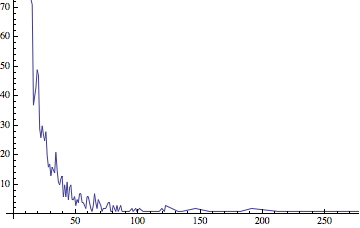
\includegraphics[width=0.4\textwidth]{FIG/indegree.png} &
     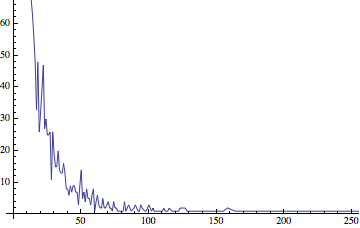
\includegraphics[width=0.4\textwidth]{FIG/outdegree.png} \\
    (a) & (b) 
\end{tabular}
\caption{In degree distribution (a) and out degree distribution (b)}
\label{fig:results}
\end{center}
\end{figure}

\begin{figure}[htbf]
\begin{center}
     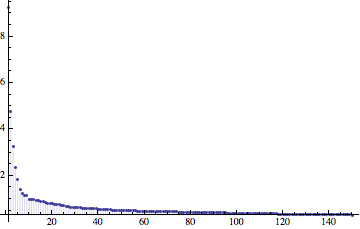
\includegraphics[width=0.6\textwidth]{FIG/pagerank.png}
\caption{Pagerank distribution}
\label{fig:pagerank}
\end{center}
\end{figure}


\begin{table}
\begin{center}
\begin{tabular}{| l | c |}
  \hline                        
  Size of WCC & Count  \\ \hline
  1 & 1384  \\ \hline
  2 & 55  \\ \hline
  3 & 1 \\ \hline
  5054 & 1 \\ \hline  
\end{tabular}
\caption{Statistics about Weakly connected components}
\label{table:wcc}
\end{center}
\end{table}

\begin{table}
\begin{center}
\begin{tabular}{| l | c |}
  \hline                        
  radius & number of vertices  \\ \hline
  0 & 1896  \\ \hline
  1 & 84  \\ \hline
  2 & 11 \\ \hline
  3 & 7 \\ \hline  
  4 & 634 \\ \hline  
  5 & 2194 \\ \hline  
  6 & 826 \\ \hline  
  7 & 117 \\ \hline  
  8 & 13 \\ \hline
  9 & 2 \\ \hline   
\end{tabular}
\caption{statistics about radius}
\label{table:radius}
\end{center} 
\end{table}

\begin{figure}[htbf]
\begin{center}
     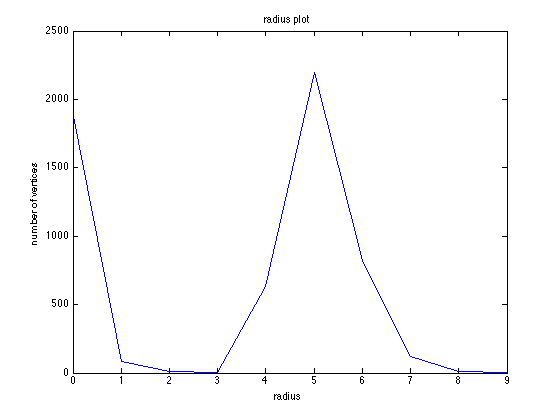
\includegraphics[width=0.6\textwidth]{FIG/radius.png}
\caption{Radius Plot}
\label{fig:radius}
\end{center}
\end{figure}

\subsection{Triangle Counting(Design)}
The main reason of triangle counting is to compare the capability of each solution(RDBMS, general purpose programming language). We will apply RDBMS version and c++/java version, record their running time and resource usage, then do performance analysis. 

\subsection{Belief Propagation(Design)}
In order to investigate the gain of using RDBMS, We plan to compare the efficiency of RDBMS's implementation of BP with BP in general purpose languages like c++/java. We ponder that the difference will be only observable in large dataset, we will conduct experiments to try to estimate that. 

\subsection{Eigenvalue/SVD(Design)}
SVD is a powerful tool at dimension reduction, or in another words, clustering. So We plan to apply SVD to social networks to find communities, and some work has been done by researchers in data mining and matrix analysis. 

\subsection{Broad Spectrum Analysis}
We apply our proposed graph mining algorithms to several real-world graph datasets from KONECT project to find global patterns and detect strange behaviors. In the following, we'll first describe the dataest then discuss  what we observe. 

\begin{description}
	\item{{\bf Route Views\cite{konect:2013:as20000102, konect:DBLP}:}}{This is an undirected network of autonomous systems of the Internet connected with each other. Nodes are autonomous systems (AS), and edges denote communication. The network contains loops. It contains 6,474 vertices and 13,895 edges.}
	\item{{\bf DBLP\cite{konect:2013:dblp-cite, konect:DBLP}:}}{This is the citation network of DBLP, a database of scientific publications such as papers and books. Each node in the network is a publication, and each edge represents a citation of a publication by another publication. In other words, the directed edge (A to B) denotes that publication A cites publication B. Publications are allowed to cite themselves, and therefore the network contains loops. It contains 12,495 vertices and 49,793 edges.}
\end{description}

We first show the degree distribution of these graphs, blah blah...

\begin{figure}[htbf]
\begin{center}
\begin{tabular}{cc}
     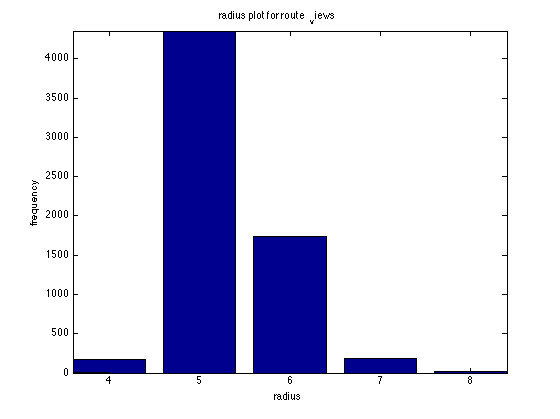
\includegraphics[width=0.4\textwidth]{FIG/route_radius.png} &
     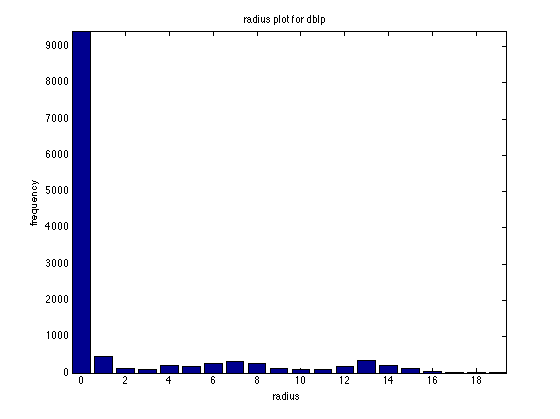
\includegraphics[width=0.4\textwidth]{FIG/dblp_radius.png} \\
    (a) & (b) 
\end{tabular}
\caption{Radius plot for Route Views (a) and Radius plot for DBLP (b)}
\label{fig:radius_plot}
\end{center}
\end{figure}

The radius plot for dataset are shown in figure \ref{fig:radius_plot}. 

From radius distribution of route views, we can see that all the vertices has radius more than 3. And since this is a connected graph (from the result we got by applying connected component algorithm), we can conclude that vertices(Autonomous Systems) with smaller radius plays a more centric role in the graph where most other vertices have direct or indirect communication (within very few hops) with. We find very few vertices with radius 4 are in the center of the graph, then most of the vertices with radius 5 are surrounding these centric vertices. Then the number of vertices decrease exponetialy as the radius grows. And finally, very few vertices (less than 20) are in the margin of the entire AS networks.  

For another graph DBLP, we observe strange behaviors. In this radius distribution, we observe that the great majority of the vertices have 0 radius, which means these papers didn't cite any other papers. We can only explain this observation by assuming all the cited papers of all those 9000 papers are not within this dataset. For other radius value, we don't observe apparent power law but rather more or less uniform distribution. However, in an exact or more complete citation graph, we should see several few popular papers pointing to each other, and has rather small radius, and most other less famous papers has longer citation path (larger radius). Therefore, we can conclude that this is a small sub-graph that don't capture the significant characteristic of a complete citation graph.


